\documentclass{article}

\usepackage{geometry}
\usepackage{xeCJK}
\usepackage{amsmath}
\usepackage{tikz}
\usepackage{pgfplots}
% figure[H] float
\usepackage{float}
% subfigure
\usepackage{subcaption}
\usepackage{amssymb}
\usepackage{hyperref}
\usepackage{setspace}
% 字体底部样式:下划线、波浪线等
\usepackage{ulem}
% 修改公式编号
\usepackage{chngcntr}

% make cdot thicker,比 cdot 更粗的圆点
\makeatletter
\newcommand*\bigcdot{\mathpalette\bigcdot@{.5}}
\newcommand*\bigcdot@[2]{\mathbin{\vcenter{\hbox{\scalebox{#2}{$\m@th#1\bullet$}}}}}
\makeatother

% 设置行间距 1.5 倍
\renewcommand{\baselinestretch}{1.5}
% 自定义图片的标题:Figure -> 图
\renewcommand{\figurename}{图}
% 自定义表格的标题:Table -> 表
\renewcommand{\tablename}{表}

% 设置页大小和页边距,或者scale=0.8
\geometry{a4paper,left=3.18cm,right=3.18cm,top=2.54cm,bottom=2.54cm}
% 兼容
\pgfplotsset{compat=1.16}
% 中文默认没有斜体和粗体格式,开启伪斜体和指定黑体;
\setCJKmainfont[AutoFakeSlant, BoldFont=SimHei]{SimSun}
\usetikzlibrary{positioning}
% area of hatch,面积阴影部分
\usetikzlibrary{patterns}
% 箭头类型
\usetikzlibrary{arrows.meta}

\hypersetup{
    colorlinks,
    citecolor=black,
    filecolor=black,
    linkcolor=black,
    urlcolor=black
}
% 定义amsmath arccot, ch, sh
\DeclareMathOperator{\arccot}{arccot}
\DeclareMathOperator{\ch}{ch}
\DeclareMathOperator{\sh}{sh}
% 每个章节后,重置公式编号
\counterwithin*{equation}{section}

% 修改公式标签引用颜色
\def\eqref#1{{\color{blue}\hypersetup{linkcolor=blue} (\ref{#1}) }}
% 修改图片标签引用的颜色
\def\figureref#1{{\color{blue}\hypersetup{linkcolor=blue} (\ref{#1}) }}
% 修改跳转标签引用的颜色
\def\linkref[#1]#2{\hyperref[#1]{\color{blue}\ #2\ }}
\def\secref#1{\hyperref[#1]{\color{blue}[\ref{#1}节]}}

% 添加 input 搜索目录
\makeatletter
\def\input@path{
  {../../latex_package/}
}
\makeatother

% 文字顶部和底部的弧度,使用自定义的包,避免输出错误字体文字和 warning 提示
\usepackage{./arcs/arcs}

\begin{document}
  \tableofcontents
  \newpage

  \part{定积分}
  \section{定积分的概念与性质}
    \subsection{定积分问题举例}
\subsubsection{曲边梯形的面积}
\paragraph{}
设$y=f(x)$在区间$[a,b]$上非负、连续。由直线$x=a, x=b, y=0$及曲线$y=f(x)$所围成的图形称为\uwave{曲边梯形},其中曲线弧称为\uwave{曲边}。矩形的高是不变的,它的面积可按公式

\begin{center}
  \text{矩形面积=高 $\times$ 底}
\end{center}
来计算。

\begin{figure}[H]
\centering
  % 曲边梯形的面积
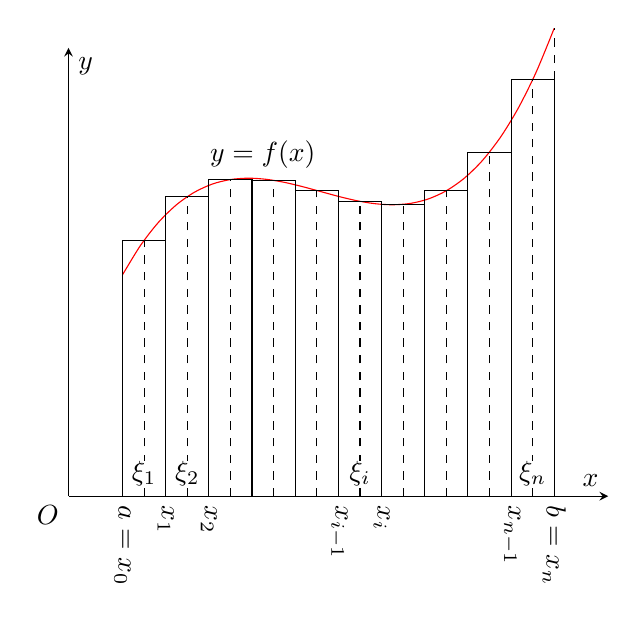
\begin{tikzpicture}[scale=1]
  \begin{axis}[clip=false,xmin=0, xmax=5,ymin=0,ymax=5, grid=none,
    xtick=\empty, ytick=\empty, axis lines=middle,
    smooth, xlabel={$x$}, ylabel={$y$}]

    % 曲线: ((x-2)**3-(x-2)**2-x)/4.0 + 4
    \addplot[draw=red,domain=0.5:4.5] {(x-2)^3/4 - (x-2)^2/4 - x/4 + 4};

    \node [above] at (1.8,3.55) {$y=f(x)$};

    \draw (0.5,0) rectangle (0.9,2.853); \draw [dashed] (0.7,0) -- (0.7,2.853);
    \draw (0.9,0) rectangle (1.3,3.34); \draw [dashed] (1.1,0) -- (1.1,3.34);
    \draw (1.3,0) rectangle (1.7,3.531); \draw [dashed] (1.5,0) -- (1.5,3.531);
    \draw (1.7,0) rectangle (2.1,3.522); \draw [dashed] (1.9,0) -- (1.9,3.522);
    \draw (2.1,0) rectangle (2.5,3.409); \draw [dashed] (2.3,0) -- (2.3,3.409);
    \draw (2.5,0) rectangle (2.9,3.288); \draw [dashed] (2.7,0) -- (2.7,3.288);
    \draw (2.9,0) rectangle (3.3,3.255); \draw [dashed] (3.1,0) -- (3.1,3.255);
    \draw (3.3,0) rectangle (3.7,3.406); \draw [dashed] (3.5,0) -- (3.5,3.406);
    \draw (3.7,0) rectangle (4.1,3.837); \draw [dashed] (3.9,0) -- (3.9,3.837);
    \draw (4.1,0) rectangle (4.5,4.644); \draw [dashed] (4.3,0) -- (4.3,4.644); \draw [dashed] (4.5,4.644) -- (4.5,5.219);

    \node [right, rotate=-90] at (0.5,0) {$a=x_0$}; \node [above,fill=white,inner sep=0.2] at (0.7,0.1) {$\xi_1$};
    \node [right, rotate=-90] at (0.9,0) {$x_1$}; \node [above,fill=white,inner sep=0.2] at (1.1,0.1) {$\xi_2$};
    \node [right, rotate=-90] at (1.3,0) {$x_2$};
    \node [right, rotate=-90] at (2.5,0) {$x_{i-1}$}; \node [above,fill=white,inner sep=0.2] at (2.7,0.1) {$\xi_i$};
    \node [right, rotate=-90] at (2.9,0) {$x_i$};
    \node [right, rotate=-90] at (4.1,0) {$x_{n-1}$}; \node [above,fill=white,inner sep=0.2] at (4.3,0.1) {$\xi_n$};
    \node [right, rotate=-90] at (4.5,0) {$b=x_n$};

    % 原点
    \node [below left] at (0,0) {$O$};
  \end{axis}
\end{tikzpicture}

  \caption{曲边梯形的面积}
  \label{曲边梯形的面积}
\end{figure}

\paragraph{}
在区间$[a,b]$中任意插入若干个分点
\begin{equation*}
  a = x_0 < x_1 < x_2 < \cdots < x_{n-1} < x_n = b,
\end{equation*}
把$[a,b]$分成$n$个小区间
\begin{equation*}
  [x_0,x_1], \; [x_1,x_2], \; \cdots, \; [x_{n-1}, x_n],
\end{equation*}
它们的长度依次为
\begin{equation*}
  \Delta x_1 = x_1 - x_0, \; \Delta x_2 = x_2 - x_1, \; \cdots, \; \Delta x_n = x_n - x_{n-1}.
\end{equation*}

\paragraph{}
因此,可求得曲边梯形面积$A$的近似值,即
\begin{align*}
  A \;\approx&\; f(\xi_1)\Delta x_1 + f(\xi_2)\Delta x_2 + \cdots + f(\xi_n)\Delta x_n \\
  =&\; \sum_{i=1}^nf(\xi_i)\Delta_i.
\end{align*}

\paragraph{}
为了保证所有小区间的长度都无限缩小,我们要求小区间长度中的最大值趋于$0$,记作$\lambda = \max|\Delta x_1, \Delta x_2, \cdots, \Delta x_n|$,则上述条件可表示为$\lambda \to 0$。当$\lambda \to 0$时(这时分段数$n$无限增多,即$n\to\infty$),取上述和式的极限,便得曲边梯形的面积

\begin{equation*}
  A = \lim_{\lambda \to 0}\sum_{i=1}^nf(\xi_i)\Delta x_i.
\end{equation*}

\subsubsection{变速直线运动的路程}
\paragraph{}
设某物体作直线运动,已知速度$v=v(t)$是时间间隔$[T_1,T_2]$上$t$的连续函数,且$v(t) \geq 0$,计算在这段时间内物体所经过的路程$s$。

\paragraph{}
对于等速直线运动,有公式
\begin{center}
  路程 = 速度 $\times$ 时间.
\end{center}

\paragraph{}
在时间间隔$[T_1,T_2]$内任意插入若干个分点
\begin{equation*}
  T_1 = t_0 < t_1 < t_2 < \cdots < t_{n-1} < t_n = T_2,
\end{equation*}
把$[T_1,T_2]$分成$n$个小时段
\begin{equation*}
  [t_0,t_1], [t_1, t_2], \cdots, [t_{n-1}, t_n],
\end{equation*}
各小时段时间的长依次为
\begin{equation*}
  \Delta t_1 = t_1 - t_0, \; \Delta t_2 = t_2 - t_1, \; \cdots, \; \Delta t_n = t_n - t_{n-1}.
\end{equation*}
相应的,在各段时间内物体经过的路程依次为
\begin{equation*}
  \Delta s_1, \Delta s_2, \cdots, \Delta s_n.
\end{equation*}
在时间间隔$[t_{i-1}, t_i]$上任取一个时刻$\tau_i \;(t_{i-1} \leq \tau_i \leq t_i)$,以$\tau_i$时的速度$v(\tau_i)$来代替$[t_{i-1}, t_i]$上各个时刻的速度,得到部分路程$\Delta s_i$的近似值,即
\begin{equation*}
  \Delta s_i \approx v(\tau_i)\Delta t_i \; (i=1,2,\cdots,n).
\end{equation*}
于是这$n$段部分路程的近似值之和就是所求变速直线运动路程$s$的近似值,即
\begin{align*}
  s \;\approx&\; v(\tau_1)\Delta t_1 + v(\tau_2)\Delta t_2 + \cdots + v(\tau_n)\Delta t_n \\
  =&\; \sum_{i=1}^nv(\tau_i)\Delta t_i.
\end{align*}
记$\lambda = \max\{\Delta t_1, \Delta t_2, \cdots, \Delta t_n\}$,当$\lambda \to 0$时,取上述和式的极限,即得变速直线运动的路程
\begin{equation*}
  s = \lim_{\lambda \to 0}\sum_{i=1}^nv(\tau_i)\Delta t_i.
\end{equation*}

\subsection{定积分定义}
\subsubsection{定义}
\paragraph{}
\textbf{定义\;}设函数$f(x)$在$[a,b]$上有界,在$[a,b]$中任意插入若干个分点
\begin{equation*}
  a = x_0 < x_1 < x_2 < \cdots < x_{n-1} < x_n = b,
\end{equation*}
把区间$[a,b]$分成$n$个小区间
\begin{equation*}
  [x_0,x_1], [x_1,x_2], \cdots, [x_{n-1},x_n],
\end{equation*}
各个小区间的长度依次为
\begin{equation*}
  \Delta x_1 = x_1 - x_0, \; \Delta x_2 = x_2 - x_1, \; \cdots, \; \Delta x_n = x_n - x_{n-1}.
\end{equation*}
在每个小区间$[x_{i-1}, x_i]$上任取一点$\xi_i \; (x_{i-1} \leq \xi_i \leq x_i)$,作函数值$f(\xi_i)$与小区间长度$\Delta x_i$的乘积$f(\xi_i)\Delta x_i \; (i=1,2,\cdots,n)$,并作出和
\begin{equation}
  S = \sum_{i=1}^n f(\xi_i)\Delta x_i,
\end{equation}
记$\lambda = \max\{\Delta x_1, \Delta x_2, \cdots, \Delta x_n\}$,如果不论对$[a,b]$怎样划分,也不论在小区间$[x_{i-1}, x_i]$上点$\xi_i$怎样选取,只要当$\lambda \to 0$时,和$S$总趋于确定的极限$I$,那么称这个极限$I$为函数$f(x)$在区间$[a,b]$上的\uwave{定积分}(简称\uwave{积分}),记作$\displaystyle\int_a^bf(x)dx$,即
\begin{equation}
  \int_a^bf(x)dx = I = \lim_{\lambda \to 0}\sum_{i=1}^nf(\xi_i)\Delta x_i,
\end{equation}
其中$f(x)$叫做\uwave{被积函数},$f(x)dx$叫做\uwave{被积表达式},$x$叫做\uwave{积分变量},$a$叫做\uwave{积分下限},$b$叫做\uwave{积分上限},$[a,b]$叫做\uwave{积分区间}。

\subsubsection{定理}
\paragraph{}
\textbf{定理1\;}设$f(x)$在区间$[a,b]$上连续,则$f(x)$在$[a,b]$上可积。

\paragraph{}
\textbf{定理2\;}设$f(x)$在区间$[a,b]$上有界,且只有有限个间断点,则$f(x)$在$[a,b]$上可积。

\subsection{定积分的近似计算}
\subsubsection{矩形法}
\paragraph{}
参考图\figureref{曲边梯形的面积},近似计算公式:
\begin{equation}
  \int_a^bf(x)dx \approx \frac{b-a}{n}(y_1+y_2+\cdots+y_n).
\end{equation}

\subsubsection{梯形法}
\paragraph{}
原理:将曲线$y=f(x)$上的小弧段$\overarc{M_{i-1}M_i}$用直线段$\overline{M_{i-1}M_i}$代替,然后用梯形代替要求的面积,由此得到定积分的近似值为
\begin{align}
\begin{split}
  \int_a^bf(x)dx \;\approx&\; \frac{b-a}{n}\big(\frac{y_0+y_1}{2} + \frac{y_1+y_2}{2} + \cdots + \frac{y_{n-1}+y_n}{2}\big) \\
  =&\; \frac{b-a}{n}\big(\frac{y_0+y_n}{2}+y_1 + y_2 + \cdots + y_{n-1}\big)
\end{split}
\end{align}

\begin{figure}[H]
\centering
  % 梯形法
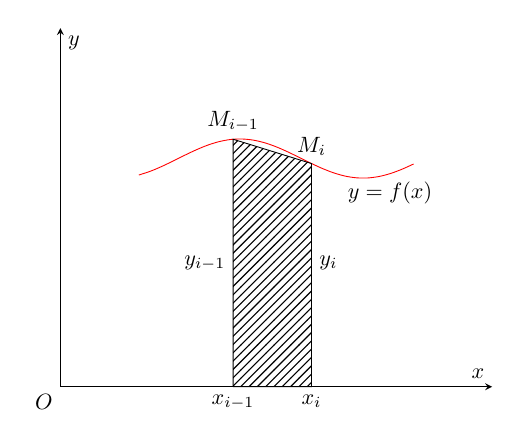
\begin{tikzpicture}[scale=0.8]
  \begin{axis}[clip=false,xmin=0, xmax=5.5,ymin=0,ymax=5.5, grid=none,
    xtick=\empty, ytick=\empty, axis lines=middle,
    smooth, xlabel={$x$}, ylabel={$y$}]

    % 曲线
    \addplot[draw=red,domain=1:4.5] {0.3*sin(deg(2*x-3)) + 3.5};

    \draw [pattern=north east lines] (2.2,0) -- (2.2,3.796) -- (3.2,3.423) -- (3.2,0) -- (2.2,0);

    \node [below] at (2.2,0) {$x_{i-1}$};
    \node [left] at (2.2,1.9) {$y_{i-1}$};
    \node [above] at (2.2,3.796) {$M_{i-1}$};

    \node [below] at (3.2,0) {$x_i$};
    \node [right] at (3.2,1.9) {$y_i$};
    \node [above] at (3.2,3.423) {$M_i$};

    \node [below] at (4.2,3.268) {$y=f(x)$};

    % 原点
    \node [below left] at (0,0) {$O$};
  \end{axis}
\end{tikzpicture}

  \caption{梯形法}
  \label{梯形法}
\end{figure}

\subsubsection{抛物线法(辛普森法)}
\paragraph{}
原理:将曲线$y=f(x)$上的两个小弧段$\overarc{M_{i-1}M_i}$和$\overarc{M_iM_{i+1}}$合并起来,用过$M_{i-1}, M_i, M_{i+1}$三点的抛物线$y = px^2+qx+r$代替。经推导得,此抛物线弧段为曲边、以$[x_{i-1},x_{i+1}]$为底的曲边梯形面积为
\begin{equation}
  \frac{1}{6}(y_{i-1}+4y_i+y_{i+1}) \bigcdot 2\Delta x = \frac{b-a}{3n}(y_{i-1} + 4y_i + y_{i+1}).
\end{equation}
取$n$为偶数,得到定积分的近似值为
\begin{align}
\begin{split}
  \int_a^bf(x)dx \;\approx&\; \frac{b-a}{3n}[(y_0+4y_1+y_2) + (y_2+4y_3+y_4) + \cdots + (y_{n-2}+4y_{n-1}+y_n)] \\
  =&\; \frac{b-a}{3n}[y_0+y_n+4(y_1+y_3+\cdots+y_{n-1}) + 2(y_2+y_4+\cdots+y_{n-2})].
\end{split}
\end{align}

\begin{figure}[H]
\centering
  \input{figure/Simpson‘s_rule}
  \caption{抛物线法}
  \label{抛物线法}
\end{figure}

\subsection{定积分的性质}
\paragraph{}
补充
\begin{enumerate}
  \item 当$a=b$时,$\displaystyle\int_a^bf(x)dx=0$;
  \item 当$a>b$时,$\displaystyle\int_a^bf(x)dx = -\int_b^af(x)dx$。
\end{enumerate}

\paragraph{}
\textbf{性质1\;}$\displaystyle\int_a^b[f(x)\pm g(x)]dx = \int_a^bf(x)dx \pm \int_a^bg(x)dx$。

\paragraph{}
\textbf{性质2\;}$\displaystyle\int_a^bkf(x)dx = k\int_a^bf(x)dx$($k$是常数)。

\paragraph{}
\textbf{性质3\;}设$a<c<b$,则积分区间具有\uwave{可加性}
\begin{equation}
  \int_a^bf(x)dx = \int_a^cf(x)dx + \int_c^bf(x)dx.
\end{equation}

\paragraph{}
\textbf{性质4\;}如果在区间$[a,b]$上$f(x)\equiv 1$,则
\begin{equation}
  \int_a^b1dx = \int_a^bdx=b-a.
\end{equation}

\paragraph{}
\textbf{性质5\;}如果在区间$[a,b]$上,$f(x)\geq 0$,则
\begin{equation}
  \int_a^bf(x)dx \geq 0 \; (a<b).
\end{equation}

\paragraph{}
\textbf{推论1\;}如果在区间$[a,b]$上,$f(x)\leq g(x)$,则
\begin{equation}
  \int_a^bf(x)dx \leq \int_a^bg(x)dx \; (a<b).
\end{equation}

\paragraph{}
\textbf{推论2\;}$\displaystyle\big| \int_a^bf(x)dx \big| \leq \int_a^b|f(x)|dx \; (a<b)$。

\paragraph{}
\textbf{性质6\;}设$M$及$m$分别是函数$f(x)$在区间$[a,b]$上的最大值及最小值,则
\begin{equation}
  m(b-a) \leq \int_a^bf(x)dx \leq M(b-a) \; (a<b).
\end{equation}

\paragraph{}
\textbf{性质7(定积分中值定理)\;}如果函数$f(x)$在积分区间$[a,b]$上连续,则在$[a,b]$上至少存在一个点$\xi$,使下式成立:
\begin{equation}
  \int_a^bf(x)dx = f(\xi)(b-a) \; (a\leq\xi\leq b).
\end{equation}
这个公式叫做\uwave{积分中值公式}。

\begin{figure}[H]
\centering
  % 定积分中值定理示例
\begin{tikzpicture}[scale=0.8]
  \begin{axis}[clip=false,xmin=0, xmax=6,ymin=0,ymax=6, grid=none,
    xtick=\empty, ytick=\empty, axis lines=middle,
    smooth, xlabel={$x$}, ylabel={$y$}]

    \addplot[draw=red,domain=1:5] {2*ln(x) + 2};

    \node [above] at (4,5.22) {$y=f(x)$};

    \draw (1,0) -- (1,2);
    \draw (5,0) -- (5,5.22);
    \draw [dashed] (3,0) -- (3,4.2);
    \draw [dashed] (0,4.2) -- (5,4.2);
    \draw [dashed] (1,0) -- (1,4.2);

    \node [below] at (1,0) {$a$};
    \node [below] at (3,0) {$\xi$};
    \node [below] at (5,0) {$b$};
    \node [left] at (0,4.2) {$f(\xi)$};

    % 原点
    \node [below left] at (0,0) {$O$};
  \end{axis}
\end{tikzpicture}

  \caption{定积分中值定理示例}
  \label{定积分中值定理示例}
\end{figure}

\paragraph{}
按积分中值公式所得函数$f(x)$在区间$[a,b]$上的\uwave{平均值}:
\begin{equation}
  f(\xi) = \frac{1}{b-a}\int_a^bf(x)dx.
\end{equation}

  \section{微积分基本公式}
    \subsection{变速直线运动中位置函数与速度函数之间的联系}
\paragraph{}
有一物体在一直线上运动。在这直线上取定原点、正向及长度单位,使它成一数轴。设时刻$t$时物体所在位置为$s(t)$,速度为$v(t)$(为了讨论方便起见,可以设$v(t) \geq 0$)。

\paragraph{}
从第一节知道:物体在时间间隔$[T_1,T_2]$内经过的路程可以用速度函数$v(t)$在$[T_1,T_2]$上的定积分

\begin{equation*}
  \int_{T_1}^{T_2}v(t)dt
\end{equation*}
来表达;另一方面,这段路程又可以通过位置函数$s(t)$在区间$[T_1,T_2]$上的增量

\begin{equation*}
  s(T_2) - s(T_1)
\end{equation*}

来表达。由此可见,位置函数$s(t)$与速度函数$v(t)$之间有如下关系:
\begin{equation}
  \label{变速直线运动速度定积分与路程关系}
  \int_{T_1}^{T_2}v(t)dt = s(T_2) - s(T_1).
\end{equation}

\paragraph{}
因为$s'(t)=v(t)$,即位置函数$s(t)$是速度函数$v(t)$的原函数,所以关系式\eqref{变速直线运动速度定积分与路程关系}表示,速度函数$v(t)$在区间$[T_1,T_2]$上的定积分等于$v(t)$的原函数$s(t)$在区间$[T_1,T_2]$上的增量
\begin{equation*}
  s(T_2) - s(T_1).
\end{equation*}

\paragraph{}
上述讨论的问题具有特殊性。因此,在\secref{sec:牛顿-莱布尼茨公式}下面进一步论证普遍性的函数$f(x)$在区间$[a,b]$上的积分等于原函数在区间$[a,b]$上的增量

\begin{equation*}
  F(b) - F(a).
\end{equation*}

\subsection{积分上限的函数及其导数}
\paragraph{}
设函数$f(x)$在区间$[a,b]$上连续,并且设$x$为$[a,b]$上的一点。我们考察$f(x)$在部分区间$[a,x]$上的定积分
\begin{equation*}
  \int_a^xf(x)dx.
\end{equation*}

\paragraph{}
由于$f(x)$在$[a,x]$上仍旧连续,因此这个定积分存在。这里,$x$即表示定积分的上限,又表示积分变量。因为定积分与积分变量的记法无关,所以,为了不混淆起见,可以把积分变量改用其它符号,例如用$t$表示,则上面的定积分可以写成

\begin{equation*}
  \int_a^xf(t)dt.
\end{equation*}

\paragraph{}
如果上限$x$在区间$[a,b]$上任意变动,则对于每一个取定的$x$值,定积分有一个对应值,所以它在$[a,b]$上定义了一个函数,记作$\Phi(x)$:
\begin{equation*}
  \Phi(x) = \int_a^xf(t)dt \; (a\leq x \leq b).
\end{equation*}

\paragraph{}
\textbf{定理1\;}如果函数$f(x)$在区间$[a,b]$上连续,则积分上限的函数
\begin{equation}
  \Phi(x) = \int_a^xf(t)dt
\end{equation}
在$[a,b]$上可导,并且它的导数
\begin{equation}
  \Phi'(x) = \frac{d}{dx}\int_a^xf(t)dt = f(x) \; (a \leq x \leq b).
\end{equation}

\paragraph{}
\textbf{证\;}若$x\in(a,b)$,设$x$获得增量$\Delta x$,其绝对值足够地小,使得$x+\Delta x\in(a,b)$,则$\Phi(x)$在$x+\Delta x$处的函数值为

\begin{equation*}
  \Phi(x+\Delta x) = \int_a^{x+\Delta x}f(t)dt.
\end{equation*}

\begin{figure}[H]
\centering
  % 积分上限的函数证明
\begin{tikzpicture}[scale=0.8]
  \begin{axis}[clip=false,xmin=0, xmax=13,ymin=0,ymax=13, grid=none,
    xtick=\empty, ytick=\empty, axis lines=middle,
    smooth, xlabel={$x$}, ylabel={$y$}]

    % 曲线:python, (x/3.5-1)**3-2*(x/3.5-1)**2+6
    \addplot[draw=red,domain=1:12] {(x/3.5-1)^3-2*(x/3.5-1)^2+8};

    \addplot[domain=1:7,pattern=north east lines,draw opacity=0] {(x/3.5-1)^3-2*(x/3.5-1)^2+8} \closedcycle;

    \node [above] at (3.4,7.956) {$y=f(x)$};

    \draw (1,0) -- (1,6.615);
    \draw (12,0) -- (12,10.53);
    \draw (7,0) -- (7,7);
    \draw [dashed] (8.5,0) -- (8.5,6.83);
    \draw (10,0) -- (10,7.51);

    \node [below] at (1,0) {$a$};
    \node [below] at (12,0) {$b$};
    \node [below] at (7,0) {$x$};
    \node [below] at (8.5,0) {$\xi$};
    \node [below] at (10.2,0) {$x+\Delta x$};
    \node [fill=white] at (8.5,3.3) {$f(\xi)$};
    \node [fill=white] at (4,3.3) {$\Phi(x)$};

    % 原点
    \node [below left] at (0,0) {$O$};
  \end{axis}
\end{tikzpicture}

  \caption{积分上限的函数证明}
  \label{积分上限的函数证明}
\end{figure}

由此得函数的增量
\begin{align*}
\Delta\Phi \;=&\; \Phi(x+\Delta x) - \Phi(x) \\
  =&\; \int_a^{x+\Delta x}f(t)dt - \int_a^xf(t)dt \\
  =&\; \int_a^xf(t)dt + \int_x^{x+\Delta x}f(t)dt - \int_a^xf(t)dt \\
  =&\; \int_x^{x+\Delta x}f(t)dt.
\end{align*}
再应用积分中值定理,即有等式
\begin{equation*}
  \Delta\Phi = f(\xi)\Delta x,
\end{equation*}
这里,$\xi$在$x$与$x+\Delta x$之间,把上式两端各除以$\Delta x$,得函数增量与自变量增量的比值
\begin{equation*}
  \frac{\Delta\Phi}{\Delta x} = f(\xi).
\end{equation*}

\paragraph{}
由于假设$f(x)$在$[a,b]$上连续,而$\Delta x \to 0$时,$\xi \to x$,因此$\displaystyle\lim_{\Delta x \to 0}=f(x)$。于是,令$\Delta x \to 0$对上式两端取极限时,左端的极限也应该存在且等于$f(x)$。这就是说,函数$\Phi(x)$的导数存在,并且
\begin{equation*}
  \Phi'(x) = f(x).
\end{equation*}

\paragraph{}
若$x=a$,取$\Delta x > 0$,则同理可证$\Phi'_+(a) = f(a)$;若$x=b$,取$\Delta x < 0$,则同理可证$\Phi'_-(b)=f(b)$。

\paragraph{}
\label{积分上限的函数}
\textbf{定理2\;}如果函数$f(x)$在区间$[a,b]$上连续,则函数
\begin{equation}
  \label{积分上限函数的定义式}
  \Phi(x)=\int_a^xf(t)dt
\end{equation}
就是$f(x)$在$[a,b]$上的一个原函数。

\subsection{牛顿-莱布尼茨公式}
\label{sec:牛顿-莱布尼茨公式}
\paragraph{}
\textbf{定理3\;}如果函数$F(x)$是连续函数$f(x)$在区间$[a,b]$上的一个原函数,则
\begin{equation}
  \label{微积分基本公式}
  \int_a^bf(x)dx = F(b) - F(a).
\end{equation}

\paragraph{}
\textbf{证\;}已知函数$F(x)$是连续函数$f(x)$的一个原函数,又根据\linkref[积分上限的函数]{定理2}知道,积分上限的函数
\begin{equation}
  \Phi(x) = \int_a^xf(t)dt
\end{equation}
也是$f(x)$的一个原函数。于是这两个原函数之差$F(x) - \Phi(x)$在$[a,b]$上必定是某一个常数$C$,即
\begin{equation}
  \label{定积分原函数之差}
  F(x) - \Phi(x) = C \; (a \leq x \leq b).
\end{equation}
在上式中令$x=a$,得$F(a) - \Phi(a) = C$。又由$\Phi(x)$的定义式\eqref{积分上限函数的定义式}可知$\Phi(a) = 0$,因此,$C=F(a)$。以$F(a)$代入\eqref{定积分原函数之差}式中的$C$,以$\displaystyle\int_a^xf(t)dt$代入\eqref{定积分原函数之差}式中的$\Phi(x)$,可得

\begin{equation}
  \int_a^xf(t)dt = F(x) - F(a).
\end{equation}

在上式中令$x=b$,就得到所要证明的公式\eqref{微积分基本公式}。

\paragraph{}
\eqref{微积分基本公式}式对$a>b$的情形同样成立。为了方便起见,以后把$F(b) - F(a)$记成$[F(x)]_a^b$,于是\eqref{微积分基本公式}式又可写成
\begin{equation}
  \int_a^bf(x)dx = [F(x)]_a^b.
\end{equation}

\paragraph{}
公式\eqref{微积分基本公式}叫做\uwave{牛顿(Newton)-莱布尼茨(Leibniz)公式},也通常叫做\uwave{微积分基本公式}。

  \section{定积分的换元法和分部积分法}
    \subsection{定积分的换元法}
\paragraph{}
\textbf{定理\;}假设函数$f(x)$在区间$[a,b]$上连续,函数$x=\varphi(t)$满足条件:
\begin{enumerate}
  \item $\varphi(\alpha) = a, \varphi(\beta) = b$;
  \item $\varphi(t)$在$[\alpha,\beta]$(或$[\beta,\alpha]$)上具有连续导数,且其值域$R_\varphi=[a,b]$,则有
  \begin{equation}
    \label{换元公式}
    \int_a^bf(x)dx = \int_\alpha^\beta f[\varphi(t)]\varphi'(t)dt.
  \end{equation}
\end{enumerate}
公式\eqref{换元公式}叫做定积分的\uwave{换元公式}。

\paragraph{}
\textbf{证\;}由假设可以知道,上式两边的被积函数都是连续的,因此不仅上式两边的定积分都存在,而且由上节的\linkref[积分上限函数的定义式]{定理2}知道,被积函数的原函数也都存在。所以,\eqref{换元公式}式两边的定积分都可应用牛顿-莱布尼茨公式。假设$F(x)$是$f(x)$的一个原函数,则
\begin{equation*}
  \int_a^bf(x)dx = F(b) - F(a).
\end{equation*}
另一方面,记$\Phi(t)=F[\varphi(t)]$,它是由$F(x)$与$x=\varphi(t)$复合而成的函数。由复合函数求导法则,得
\begin{equation*}
  \Phi'(t) = \frac{dFdx}{dxdt} = f(x)\varphi'(t) = f[\varphi(t)]\varphi'(t).
\end{equation*}
这表明$\Phi(t)$是$f[\varphi(t)]\varphi'(t)$的一个原函数。因此有
\begin{equation*}
  \int_\alpha^\beta f[\varphi(t)]\varphi'(t)dt = \Phi(\beta) - \Phi(\alpha).
\end{equation*}
又由$\Phi(t)=F[\varphi(t)]$及$\varphi(\alpha) = a, \varphi(\beta) = b$可知
\begin{equation*}
  \Phi(\beta) - \Phi(\alpha) = F[\varphi(\beta)] - F[\varphi(\alpha)] = F(b) - F(a).
\end{equation*}
所以
\begin{align*}
  \int_a^bf(x)dx \;=&\; F(b) - F(a) = \Phi(\beta) - \Phi(\alpha) \\
  =&\; \int_\alpha^\beta f[\varphi(t)]\varphi'(t)dt.
\end{align*}
这就证明了换元公式。

\paragraph{}
换元公式也可反过来使用。为使用方便起见,把换元公式中左右两边对调位置,同时把$t$改记为$x$,而$x$改记为$t$,得
\begin{equation}
  \int_a^bf[\varphi(x)]\varphi'(x)dx = \int_\alpha^\beta f(t)dt.
\end{equation}
这样,我们可用$t=\varphi(x)$来引入新变量$t$,而$\alpha = \varphi(a), \beta = \varphi(b)$。

\subsection{定积分的分部积分法}
\paragraph{}
依据不定积分的分部积分法,可得
\begin{align}
\begin{split}
  \int_a^bu(x)v'(x)dx \;=&\; \big[ \int u(x)v'(x)dx \big]_a^b \\
    =&\; \big[ u(x)v(x) - \int v(x)u'(x)dx \big]_a^b \\
    =&\; \big[ u(x)v(x) \big]_a^b - \int_a^b v(x)u'(x)dx,
\end{split}
\end{align}
简记作
\begin{equation}
  \int_a^buv'dx = [uv]_a^b - \int_a^bvu'dx,
\end{equation}
或
\begin{equation}
  \int_a^budv = [uv]_a^b - \int_a^bvdu.
\end{equation}
这就是\uwave{定积分的分部积分公式}。公式表明原函数已经积出的部分可以先用上、下限代入。

  \section{反常积分}
    \paragraph{}
在一些实际问题中,常会遇到积分区间为无穷区间,或者被积函数为无界函数的积分,它们已经不属于前面所说的定积分了。因此,我们对定积分作如下两种推广,从而形成\uwave{反常积分}的概念。

\subsection{无穷限的反常积分}
\paragraph{}
\textbf{定义1\;}设函数$f(x)$在区间$[a,+\infty)$上连续,取$t>a$,如果极限
\begin{equation}
  \lim_{t \to +\infty} \int_a^tf(x)dx
\end{equation}
存在,则称此极限为\uwave{函数{$f(x)$}在无穷区间{$[a,+\infty)$}上的反常积分},记作$\displaystyle\int_a^{+\infty}f(x)dx$,即

\begin{equation}
  \int_a^{+\infty}f(x)dx = \lim_{t \to +\infty}\int_a^tf(x)dx,
\end{equation}
这时也称\uwave{反常积分}$\displaystyle\int_a^{+\infty}f(x)dx$\uwave{收敛};如果上述极限不存在,则函数$f(x)$在无穷区间$[a,+\infty)$上的反常积分$\displaystyle\int_a^{+\infty}f(x)dx$就没有意义,习惯上称为\uwave{反常积分}$\displaystyle\int_a^{+\infty}f(x)dx$\uwave{发散},这时记号$\displaystyle\int_a^{+\infty}f(x)dx$不再表示数值了。

\paragraph{}
类似地,函数$f(x)$在区间$(-\infty,b]$或$(-\infty,+\infty)$上也存在相同概念。

\paragraph{}
上述反常积分统称为\uwave{无穷限的反常积分}。

\subsection{无界函数的反常积分}
\paragraph{}
如果函数$f(x)$在点$a$的任一领域内都无界,那么点$a$称为函数$f(x)$的\uwave{瑕点}(也称为无界间断点)。无界函数的反常积分又称为\uwave{瑕积分}。

\textbf{定义2\;}设函数$f(x)$在$(a,b]$上连续,点$a$为$f(x)$的瑕点。取$t>a$,如果极限
\begin{equation}
  \lim_{t \to a^+}\int_t^bf(x)dx
\end{equation}
存在,则称此极限为\uwave{函数{$f(x)$}在{$(a,b]$}上的反常积分},仍然记作$\displaystyle\int_a^bf(x)dx$,即
\begin{equation}
  \int_a^bf(x)dx = \lim_{t \to a^+}\int_t^bf(x)dx.
\end{equation}
这时也称\uwave{反常积分}$\displaystyle\int_a^bf(x)dx$\uwave{收敛}。如果上述极限不存在,则称\uwave{反常积分}$\displaystyle\int_a^bf(x)dx$\uwave{发散}。

\paragraph{}
类似地,可得到函数$f(x)$在$[a,b)$上的反常积分定义。

\paragraph{}
设函数$f(x)$在$[a,b]$上除点$c \; (a<c<b)$外连续,点$c$为$f(x)$的瑕点。如果两个反常积分

\begin{equation}
  \int_a^cf(x)dx \;\text{与}\; \int_c^bf(x)dx
\end{equation}
都收敛,则定义

\begin{align}
\begin{split}
  \int_a^bf(x)dx \;=&\; \int_a^cf(x)dx + \int_c^bf(x)dx \\
  =&\; \lim_{t \to c^-}\int_a^tf(x)dx + \lim_{t\to c^+}\int_t^bf(x)dx;
\end{split}
\end{align}
否则,就称\uwave{反常积分}$\displaystyle\int_a^bf(x)dx$\uwave{发散}。

  \section{反常积分的审敛法 $\Gamma$函数}
    \paragraph{}
本节中我们来建立不通过被积函数的原函数判断反常积分收敛性的判定法。

\subsection{无穷限反常积分的审敛法}
\paragraph{}
\textbf{定理1\;}设函数$f(x)$在区间$[a,+\infty)$上连续,且$f(x) \geq 0$。若函数
\begin{equation}
  F(x) = \int_a^xf(t)dt
\end{equation}
在$[a,+\infty)$上有上界,则反常积分$\displaystyle\int_a^{+\infty}f(x)dx$收敛。

\paragraph{}
按照“$[a,+\infty)$上的单调有界函数$F(x)$必有极限$\displaystyle\lim_{x \to +\infty}F(x)$”的准则,可证。

\paragraph{}
\textbf{定理2(比较审敛原理)\;}设函数$f(x), g(x)$在区间$[a,+\infty)$上连续。如果$0 \leq f(x) \leq g(x) \; (a \leq x < +\infty)$,并且$\displaystyle\int_a^{+\infty}g(x)dx$收敛,则$\displaystyle\int_a^{+\infty}f(x)dx$也收敛;如果$0\leq g(x) \leq f(x) \; (a \leq x < +\infty)$,并且$\displaystyle\int_a^{+\infty}g(x)dx$发散,则$\displaystyle\int_a^{+\infty}f(x)dx$也发散。

\paragraph{}
\textbf{定理3(比较审敛法1)\;}设函数$f(x)$在区间$[a,+\infty) \; (a>0)$上连续,且$f(x) \geq 0$。如果存在常数$M > 0$及$p > 1$,使得$\displaystyle f(x) \leq \frac{M}{x^p} \; (a \leq x < +\infty)$,则反常积分$\displaystyle\int_a^{+\infty}f(x)dx$收敛;如果存在常数$N > 0$,使得$\displaystyle f(x) \geq \frac{N}{x} \; (a \leq x < +\infty)$,则反常积分$\displaystyle\int_a^{+\infty}f(x)dx$发散。

\paragraph{}
\label{极限审敛法1}
\textbf{定理4(极限审敛法1)\;}设函数$f(x)$在区间$[a, +\infty)$上连续,且$f(x) \geq 0$。如果存在常数$p > 1$,使得$\displaystyle\lim_{x \to +\infty}x^pf(x)$存在,则反常积分$\displaystyle\int_a^{+\infty}f(x)dx$收敛;如果$\displaystyle\lim_{x \to +\infty}xf(x)=d > 0$(或$\displaystyle\lim_{x\to+\infty}xf(x) = +\infty$),则反常积分$\displaystyle\int_a^{+\infty}f(x)dx$发散。

\paragraph{}
\textbf{定理5\;}设函数$f(x)$在区间$[a,+\infty)$上连续。如果反常积分
\begin{equation}
  \int_a^{+\infty}|f(x)|dx
\end{equation}
收敛,则反常积分
\begin{equation}
  \int_a^{+\infty}f(x)dx
\end{equation}
也收敛。

\paragraph{}
通常称满足定理5条件的反常积分$\displaystyle\int_a^{+\infty}f(x)dx$为\uwave{绝对收敛}。于是,定理5可简单地表达为:\textbf{绝对收敛的反常积分$\displaystyle\int_a^{+\infty}f(x)dx$必定收敛}。

\subsection{无界函数的反常积分的审敛法}
\paragraph{}
\label{比较审敛法2}
\textbf{定理6(比较审敛法2)\;}设函数$f(x)$在区间$(a,b]$上连续,且$f(x) \geq 0, x = a$为$f(x)$的瑕点。如果存在常数$M > 0$及$q < 1$,使得
\begin{equation}
  f(x) \leq \frac{M}{(x-a)^q} \; (a < x \leq b),
\end{equation}
则反常积分$\displaystyle\int_a^bf(x)dx$收敛;如果存在常数$N > 0$,使得
\begin{equation}
  f(x) \geq \frac{N}{x-a} \; (a<x\leq b),
\end{equation}
则反常积分$\displaystyle\int_a^bf(x)dx$发散。

\paragraph{}
\textbf{定理7(极限审敛法2)\;}设函数$f(x)$在区间$(a,b]$上连续,且$f(x) \geq 0, x = a$为$f(x)$的瑕点。如果存在常数$0 < q < 1$,使得
\begin{equation}
  \lim_{x \to a^+}(x-a)^qf(x)
\end{equation}
存在,则反常积分$\displaystyle\int_a^bf(x)dx$收敛;如果
\begin{equation}
  \lim_{x \to a^+}(x-a)f(x) = d > 0 \; (\text{或} \lim_{x \to a^+}(x-a)f(x) = +\infty),
\end{equation}
则反常积分$\displaystyle\int_a^bf(x)dx$发散。

\subsection[Γ函数]{$\Gamma$函数}
\paragraph{}
$\Gamma$函数的定义:
\begin{equation}
  \label{Gamma 函数定义}
  \Gamma(s) = \int_0^{+\infty}e^{-x}x^{s-1}dx \; (s > 0).
\end{equation}

\begin{figure}[H]
\centering
  % Gamma 函数
\psset{unit=1cm}
\begin{pspicture*}(-1,-1)(5,5)
  % 坐标
  \psaxes[showorigin=false,linewidth=.5pt,ticksize=3pt 0]{->}(0,0)(0,0)(5,5)[$ s $, -120][$ \Gamma(s) $, -140]
  % 原点标签
  \rput[tr](-.1,-.1){$O$}
  % 设置画线的样式
  \psset{linecolor=red,linewidth=.5pt,plotpoints=100,algebraic}
  % Gamma 函数
  \psplot{.2}{3.75}{GAMMA(x)}
\end{pspicture*}

  \caption{Gamma 函数}
  \label{Gamma 函数}
\end{figure}

\paragraph{}
首先讨论\eqref{Gamma 函数定义}式右端积分的收敛性问题。这个积分区间为无穷,又当$s-1<0$时$x=0$是被积函数的瑕点。为此,分别讨论下列两个积分的收敛性:
\begin{align*}
  I_1 \;=&\; \int_0^1e^{-x}x^{s-1}dx, \\
  I_2 \;=&\; \int_1^{+\infty}e^{-x}x^{s-1}dx
\end{align*}

\paragraph{}
先讨论$I_1$,当$s \geq 1$时,$I_1$是定积分;当$0 < s < 1$时,因为
\begin{equation}
  e^{-x} \bigcdot x^{s-1} = \frac{1}{x^{1-s}} \bigcdot \frac{1}{e^x} < \frac{1}{x^{1-s}},
\end{equation}
而$1-s < 1$,根据\linkref[比较审敛法2]{比较审敛法2},反常积分$I_1$收敛。

\paragraph{}
再讨论$I_2$。因为
\begin{equation}
  \lim_{x \to +\infty}x^2 \bigcdot (e^{-x}x^{s-1}) = \lim_{x \to +\infty}\frac{x^{s+1}}{e^x} = 0,
\end{equation}
根据\linkref[极限审敛法1]{极限审敛法1},$I_2$也收敛。

\paragraph{}
由以上讨论即得反常积分$\displaystyle\int_0^{+\infty}e^{-x}x^{s-1}dx$对$s>0$均收敛。

\subsubsection{性质}
\paragraph{}

\begin{enumerate}
  \item \textbf{递推公式\;} $\Gamma(s+1)=s\Gamma(s) \; (s > 0)$。
  \item 当$s\to 0^+$时,$\Gamma(s) \to +\infty$。
  \item \textbf{余元公式\;} $\displaystyle\Gamma(s)\Gamma(1-s)=\frac{\pi}{\sin\pi s} \; (0 < s < 1)$。
  \item 在$\displaystyle\Gamma(s) = \int_0^{+\infty}e^{-x}x^{s-1}dx$中,作代换$x=u^2$,有
  \begin{equation}
    \label{Gamma函数性质4公式}
    \Gamma(s) = 2\int_0^{+\infty}e^{-u^2}u^{2s-1}du.
  \end{equation}
  再令$2s-1=t$或$\displaystyle s=\frac{1+t}{2}$,即有
  \begin{equation}
    \int_0^{+\infty}e^{-u^2}u^tdu = \frac{1}{2}\Gamma\big( \frac{1+t}{2} \big) \; (t > -1).
  \end{equation}
  上式左端是应用上常见的积分,它的值可以通过上式用$\Gamma$函数计算出来。
\end{enumerate}

\paragraph{}
在\eqref{Gamma函数性质4公式}中,令$\displaystyle s=\frac{1}{2}$,得
\begin{equation}
  2\int_0^{+\infty}e^{-u^2}du = \Gamma(\frac{1}{2}) = \sqrt{\pi}.
\end{equation}
从而
\begin{equation}
  \int_0^{+\infty}e^{-u^2}du=\frac{\sqrt{\pi}}{2}.
\end{equation}
上式左端的积分是在概率论中常用的积分。

\end{document}
